\documentclass[a4paper, 11pt]{report} %twoside
\title{Programación, Redes y Código Libre}
\author{David Davó}
\date{\today{}}

%%Packages
\usepackage[utf8]{inputenc} %Para saber el encoding del archivo
\usepackage[T1]{fontenc}
%\usepackage[no-math]{fontspec} %Para usar fuentes del sistema
\usepackage{fontspec}

\usepackage[xindy, nomain, acronym, nonumberlist, nopostdot]{glossaries}
\usepackage{glossary-mcols}

\usepackage{graphicx} %Para insertar gráficos
\usepackage{float} %PAra posicionar bien los gráficos
\usepackage{unicode-math} %Para símbolos matemagicos
%\setmathfont{Asana-Math.otf}
\setmathfont{Arial}
\usepackage[type={CC}, modifier={by-sa}, version={4.0}]{doclicense} %Muestra la licencia
\usepackage[usenames,svgnames,table]{xcolor} %Para darle color
\usepackage{dirtytalk} %Usado para citar
\usepackage{csquotes} %lo mismo qu eel anterior pero con estilo
\usepackage[spanish]{babel} %Hace que el idioma de los defaults esté en Español
\usepackage{fancyhdr} %Para poner encabezados y pies de página
%De la bibliografía y las citas.
\usepackage[
backend=biber
]{biblatex}
\addbibresource{Bibl.bib}

%Decoraciones y formato del texto
\usepackage[left=2.75cm, right=2cm, top=3cm, bottom=3cm]{geometry}

\usepackage[cache=false]{minted} %Para insertar código

\usepackage{tabularx} %Para hacer tablas muy bonicas
\usepackage{multirow}

\setmainfont{Arial}
\setmonofont{Inconsolata}
\fontsize{11}{14}
%Pies de pagina y eso
\pagestyle{fancy}
\fancyhf{}
\makeatletter
\fancyhead[LE, RO]{\@author}
\fancyhead[RE, LO]{\@title}
\fancyfoot[LE, RO]{\thepage}
\fancyfoot[C]{\leftmark}

\makeglossaries
\newglossaryentry{Libr}
{
	name=Librería,
	description={En informática, una librería o biblioteca es un conjunto de recursos y fucniones diseñadas para ser usadas por otros programas. Incluyen plantillas, funciones y clases, subrutinas, código escrito, variables predefinidas...},
	plural=librerías,
}
\newglossaryentry{datos}{
	name=Datos,
	description={Secuencia binaria de unos y ceros que contiene información codificada},
	plural=Datos, 
}
\newacronym{gnu}{GNU}{\textit{GNU's Not Unix} (GNU no es Unix)}
\newglossaryentry{Linux}
{
  name=Linux,
  description={is a generic term referring to the family of Unix-like
               computer operating systems that use the Linux kernel},
  plural=Linuces
}
\newglossaryentry{conmutacion de paquetes}{
	name={Conmutación de paquetes},
	description={Método para enviar datos por una red de computadoras. Se divide el paquete en dos partes, una con información de control que leen los nodos para enviar el paquete a su destino y los datos a enviar},
}
\newacronym{osi}{OSI}{\textit{Open Systems Interconnection} (Interconexión de Sistemas Abiertos)}
\newglossaryentry{gls-ISO}{
	name={\textit{International Organization for Standardization}},
	description={Organización Internacional de Normalización. Compuesta de varias organizaciones nacionales se encarga de la creación de estándares internacionales desde 1947.},
}
\newacronym[see={[Glossary:]{gls-ISO}}]{iso}{ISO}{\textit{International Organization for Standardization}\glsadd{gls-ISO}}
\newglossaryentry{capas de abstraccion}{
	name={capas de abstracción},
	description={Método de ocultar detalles de implementación de un set de funcionalidades},
}
\newacronym{IEEE}{IEEE}{Instituto de Ingeniería Eléctrica y Electrónica}
\newglossaryentry{topologia de red}{
	name={topología de red},
	description={Configuración espacial o física de la red. (Ver \ref{topdred} pág.\pageref{topdred})},
	plural={topologías de red},
	see={topologia}
}
\newglossaryentry{topologia}{
	name={topología},
	description={``Rama de las matemáticas que trata especialmente de la continuidad y de otros conceptos más generales originados de ella, como las propiedades de las figuras con independencia de su tamaño o forma." \cite{rae}[Topología]},
	plural={topologías},
}
\newglossaryentry{hardware}{
	name={hardware},
	description={Conjunto de elementos físicos o materiales que constituyen un sistema informático.},
}
\newacronym{MAC}{MAC}{\textit{Media Access Control}, Control de Acceso al Medio}
\newacronym{ADSL}{ADSL}{\textit{Asymmetric Digital Subscriber Line} [Línea de Abonado Digital Asimétrica]}
\newacronym{LAN}{LAN}{\textit{Local Area Network} [Red de Área Local]}
\newacronym{FTTH}{FTTH}{\textit{Fiber To The Home} [Fibra hasta el hogar]}
\newacronym[see={[Glossary:]{gls-FTTx}}]{FTTx}{FTTx}{\textit{Fiber to the X \glsadd{gls-FTTx}}}
\newglossaryentry{gls-FTTx}{
	name={FTTx},
	description={Término que agrupa las distintas configuraciones de acometida de la fibra óptica.},
}
\newglossaryentry{bit}{
	name={bit},
	description={\textit{\textbf{Bi}nary digi\textbf{t}, o dígito binario. Cada dígito del sistema de numeración binario}},
	plural={bits}
}
\newacronym{POP3}{POP3}{\textit{Post Office Protocol}, Protocolo de Oficina Postal}
\newacronym{url}{URL}{\textit{Uniform Resource Identifier}, Identificador de Recursos Uniforme}
\newglossaryentry{cache}{
	name={caché},
	description={Almacenamiento temporal de datos con el objetivo de reducir el retardo, la carga de los servidores y el ancho de banda consumido},
}
\newglossaryentry{programacion imperativa}{
	name={programación imperativa},
	description={Las órdenes del programa cambian el estado de este mismo. Por ejemplo, una variable no tiene por que ser declarada con antelación y su valor es modificable. Es la que usa el código máquina de los ordenadores},
}
\newglossaryentry{botnet}{
	name={botnet},
	description={Grupo de ordenadores coordinados conectados a un maestro mediante un virus. Gracias a este virus se pueden realizar tareas masivas como el envío de SPAM o ataques DDoS},
}
\newglossaryentry{bug}{
	name={bug},
	plural={bugs},
	description={Error en un programa informático.},
}
\newglossaryentry{repositorio}{
	name={repositorio},
	plural={repositorios},
	description={Servidor donde se alojan ficheros o archivos para su descarga},
}
\newglossaryentry{dependencia}{
	plural={dependencias},
	name={dependencia},
	description={De un programa, otro tipo de software necesario para que éste funcione}
}
\newacronym{FSF}{FSF}{\textit{Free Software Foundation}, Fundación del Software Libre}
\newacronym{IDE}{IDE}{Entorno de Desarrollo Integrado, \textit{Integrated Development Enviroment}}
\newacronym{GUI}{GUI}{Interfaz Gráfica de Usuario, \textit{Graphic User Interface})}

%%% Algunas macros
\newcommand{\acr}[1]{\acrshort{#1} (\acrlong{#1})}

%Document
\begin{document}
\makeatletter
\begin{titlepage}
\centering
\vspace*{4cm}
{\scshape\LARGE IES Palas Atenea \par}
\vspace{1cm}
{\scshape\Large Proyecto de Investigación Bachillerato de excelencia\par}
\vspace{1.5cm}
{\huge\bfseries \@title\par}
\rule{0.5\textwidth}{1pt}\par
\vspace{2cm}
{\Large\itshape \@author\par}
\vfill
Tutor\par
Julio Sánchez

\vfill

{\large \@date\par}
\pagenumbering{gobble}
\end{titlepage}
\clearpage

\tableofcontents
\newpage{}
\pagenumbering{arabic}

\chapter{Programación y código libre}

\subsection*{Propuesta}
El objetivo es el desarrollo de un software programado en Python de código libre con el que los alumnos puedan aprender tanto sobre redes como de programación en Python.

\section{Herramientas}
El programa ha sido creado con herramientas de software libre. Según la Free Software Foundation
\say{«Software libre» es el software que respeta la libertad de los usuarios y la comunidad. A grandes rasgos, significa que los usuarios tienen la libertad de ejecutar, copiar, distribuir, estudiar, modificar y mejorar el software. Es decir, el «software libre» es una cuestión de libertad, no de precio. Para entender el concepto, piense en «libre» como en «libre expresión», no como en «barra libre». En inglés a veces decimos «libre software», en lugar de «free software», para mostrar que no queremos decir que es gratuito.}
--\cite{FSF-Ph}

Todas las herramientas citadas a continuación, son o están basadas en Software Libre.

\subsection{GNU/Linux}
También llamado incorrectamente sólo Linux, es una manera de llamar al Sistema Operativo (OS) combinación del kernel Linux (Basado en Unix) y el OS \gls{gnu}, ambos software son libres y de código abierto. Normalmente Linux se distribuye en distribuciones o 'distros', las cuales contienen paquetes de software preinstalados, dependiendo del grupo de usuarios al que este dirigida.

\subsubsection*{Distros}

\subsection{Git y Github}
Git es un software diseñado por Linus Torvalds con el que puedes crear un Sistema de Control de Versiones o VCS (\textit{Version Control System}). Este programa te permite de forma sencilla volver a una versión o \textit{commit} anterior del programa, así como enviarlas a un repositorio remoto e incluso publicarlas en línea. Su punto fuerte son las \textit{branches} o ``ramificaciones" del código, haciendo que la rama \textit{master} (principal) siempre pueda ser usada. Para ello creamos una nueva rama para cada nueva funcionalidad del programa. La implementación del nuevo código a otra rama se denomina \textit{merge}.

%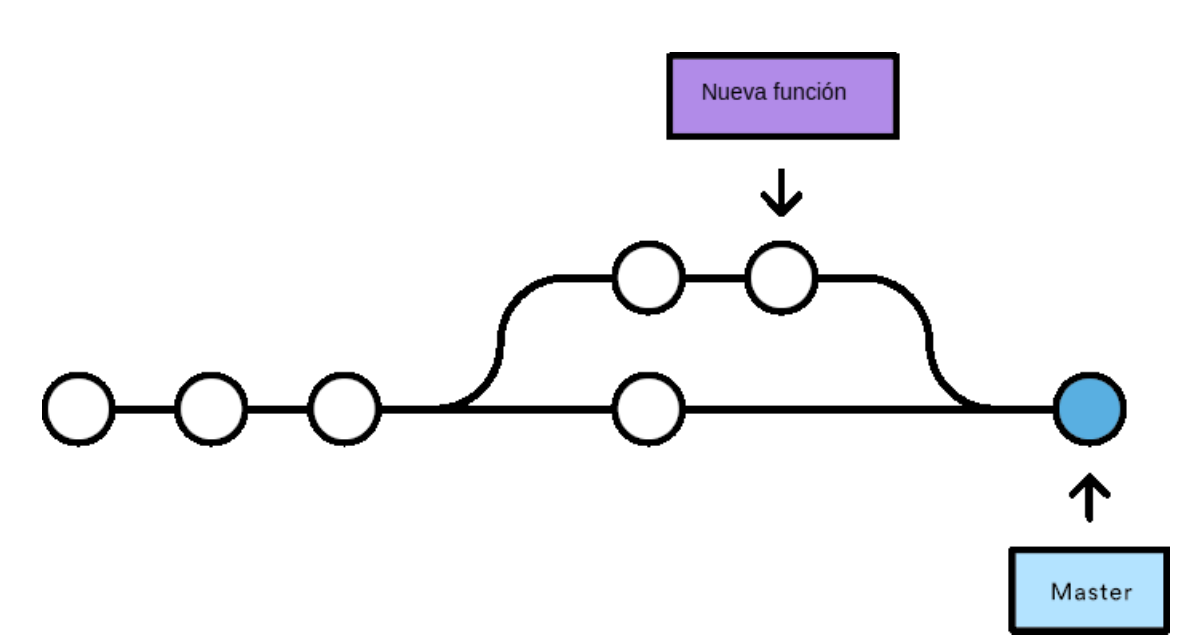
\includegraphics[width=\textwidth]{Resources/01.01.02-01.png}
\begin{figure}
\noindent
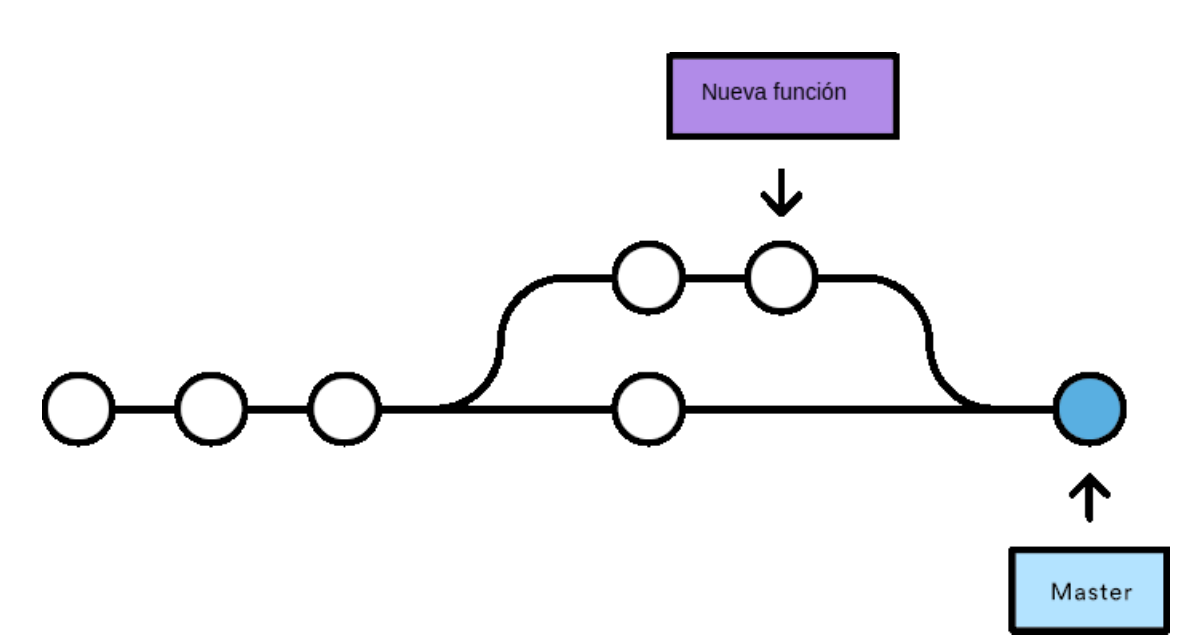
\includegraphics[width=0.95\textwidth]{Resources/01.01.02-01.png}
\caption{\textit{Branching} con Git}
\end{figure}

GitHub es una plataforma de desarrollo colaborativo que te permite alojar tus repositorios Git. Su uso es gratuito si el código almacenado es público. Además, te permite tener, una wiki y una página web para tu proyecto, junto a otras funciones.
Tanto el programa como este documento están disponibles en GitHub en el siguiente enlace. \url{https://github.com/daviddavo/InvProy}

\subsection{LaTeX}
\LaTeX\space o, en texto plano, LaTeX, pronunciado con la letra griega 
Ji ($\Chi$), es un software libre orientado a la creación de textos escritos comparable a la calidad tipográfica de las editoriales. Mediante la importación de paquetes y comandos o macros se puede dar formato al texto al igual que con cualquier otro editor, exportándolo posteriormente a PostScript o PDF. Está orientado a documentos técnicos y científicos por su facilidad a la hora de incluir fórmulas e importar paquetes que cumplan tus necesidades. No es un procesador de textos, pues está más enfocado en el contenido del documento que en la aparencia de éste.
El código del documento puede ser editado con cualquier editor de texto plano como \textit{nano} o \textit{emacs}, pero he usado una IDE llamada \textbf{texmaker}.

\subsection{Python}
Es un lenguaje de programación interpretado (sólo traducen el programa a código máquina cuando se debe ejecutar esa parte del código, por lo que no hace falta compilarlo) que destaca por pretender una sintaxis más legible que la de el resto de lenguajes. Soporta tanto programación imperativo como programación orientada a objetos. Usa variables dinámicas, es multiplataforma, y, además, es de código abierto, lo que me permite distribuir el programa en Windows al distribuir los binarios de Python junto a él. En este caso, la versión de Python usada es la 3.4 en adelante.

\subsection{Gtk+}
Es un conjunto de bibliotecas o \glspl{Libr} (conjunto de funciones y clases ya definidas preparadas para el uso de los programadores) desarrollado por la GNOME foundation destinado a la creación de GUIs (Interfaz Gráfica de Usuario), también, al igual que Linux forma parte del proyecto GNU.

Contiene las bibliotecas de GTK, GDK, ATK, Glib, Pango y Cairo; de las que he usado fundamentalmente GTK para crear la interfaz principal del programa; GDK al usarlo como intermediario entre los gráficos de bajo nivel y alto nivel y Cairo para la creación de algunos de los elementos gráficos del programa.

Al usar este conjunto de librerías, he conseguido que sólo sea necesario descargar una dependencia del programa, que además suele venir instalada en la mayoria de distros de Linux, por ejemplo en una instalación limpia de Ubuntu 16 (sin descargar paquetes adiccionales) el programa funciona perfectamente. Para usarlo en Python se ha tenido que importar la libreria de PyGtk.
\subsection{Atom}
Atom es un editor de código multiplataforma con soporte para plugins escrito en Node.js, también tiene soporte para Git. También es un programa de código libre haciendo uso de la licencia MIT.

\subsection{Wireshark}
Wireshark es un \textit{packet sniffer} o analizador de paquetes. Te muestra los paquetes de red reales enviados y recibidos por una tarjeta de red, lo que facilita la creación del simulador de redes.

\chapter{Redes Informáticas}
\section*{Historia}
Internet, tal y como lo conocemos ahora, haciendo uso de IPv6, HTML5, CSS3 no existe hasta hace recientemente, pero el desarrollo de éste transcurre desde los años 60. En 1961 se publican los primeros artículos de \gls{conmutacion de paquetes}
\section{Capas de Red/Modelo OSI}
El modelo \acr{osi} es un modelo de referencia para redes basado en \gls{capas de abstraccion}
El objetivo del modelo \gls{osi} es conseguir la interoperabilidad entre sistemas con la protocolos estandarizados. Fue creado en 1980 por la \acr{iso}. No es considerado una arquitectura de red porque los protocolos no forman parte del modelo en sí, sino son entidades de distintas normativas internacionales.
\vspace{1pt}
\definecolor{odd}{HTML}{FFFFFF}
\definecolor{even}{HTML}{E0E0E0}
\definecolor{header}{HTML}{42A5F5}

\rowcolors{1}{header}{header}
\rowcolors{2}{odd}{even}
\renewcommand{\arraystretch}{1.2}
\noindent
\begin{tabularx}{\columnwidth}{|l c X p{2cm}|}
	\rowcolor{header} \hline
	\textbf{Capa} & \textbf{PDU} & \textbf{Función} & \textbf{Ejemplos} \\ \hline
	1. Física & Bit & Transmisión y recepción de bits físicos sobre un medio físico (topología de red) & 	 RJ45, IEEE 802.11, etc. \\
	\label{osi}
	2. Data Link & Frame & Transmisión segura de \textit{frames} entre dos nodos conectados por una capa física. & Ethernet, 802.11, etc...\\
	3. Red & Paquete & Estructurar y administrar una red multinodo. Incluye enrutamiento, control de tráfico, y asignación de direcciones & IPv4, IPv6, ICMP... \\
	4. Transporte & \begin{tabular}[t]{@{}c@{}}Datagrama(UDP)\\Segmento(TCP)  \end{tabular} &
	Transmisión de segmentos de datos entre los puntos de una red, incluyendo ACK & TCP, UDP...\\
	5. Sesión & Datos & Administración de sesiones de comunicación, como intercambio continúo de información entre dos nodos. & SSH, RPC, PAP...\\ 
	6. Presentación & Datos & Translación de datos entre un servicio de red y una aplicación. Incluye comprensión, encriptación/decriptación, y codificación de carácteres. & MIME, TLS \\
	7. Aplicación & Datos & APIs de alto nivel, incluyendo recursos compartidos y acceso remoto de archivos & HTTP, FTP, SMTP... \\ \hline
\end{tabularx}

\section{Elementos físicos de una red}
Servidor, cliente, switch, hub, router, etc...

\section{Topologías de red}
\label{topdred}
La \gls{topologia} de red es la configuración de los elementos que componen una red. Puede ser representada lógica o físicamente. La topología lógica puede ser igual en dos redes, aunque su topología física (distancia entre conexiones, tipo de señales...) pueda ser distinta. Se distinguen dos elementos: los nodos (Ordenadores, switches, etc.) y los enlaces (medio de transmisión de los datos).
\subsection{Clasificación de las topologías de red}
Se distinguen ocho tipos de topologías de red: \cite{bicsi-02}
\begin{description}
\item \textbf{Punto a punto:} conexión directa entre los dos puntos de la red. También es conocida como \textit{P2P} (\textit{Peer to Peer}).
\item \textbf{Estrella:} cada host se conecta a un hub central con una conexión P2P. Cada nodo está conectado a un nodo central que puede ser un router, hub o switch.
\item \textbf{Bus:} cada nodo está conectado a un sólo cable. Una señal de un dispositivo viaja en ambos sentidos por el cable hasta que encuentra el destino deseado.
\item \textbf{Anillo:} es una topología en bus pero con los extremos conectados. Los datos atraviesan el anillo en una única dirección y van atravesando cada uno de los nodos, por lo que si uno de ellos no funciona, la red tampoco.
\item \textbf{Malla:} se pueden distinguir dos tipos: completamente conectados, en la que todos los nodos están conectados entre ellos y parcialmente conectados, en la que algunos nodos pueden estar conectados punto a punto y otros pueden tener varias conexiones.
\item \textbf{Híbrida:} combinan dos o más topologías. La más famosa es la topología de \textbf{árbol}, en la que se conectan varias topologías de estrella mediante bus. 
\item \textbf{Cadena:} se conecta cada ordenador en serie con el siguiente. Cada ordenador repite el mensaje al siguiente ordenador si éste no es su destino. Si se cierra el circuito se crea una topología en anillo, mientras que si se deja abierto se denomina topología linear.
\end{description}

\subsection{Nodos de una red}
\begin{description}
\item \textbf{\textit{Router} o enrutador:} es un dispositivo de red que reenvía los paquetes mirando en la capa 3 del modelo OSI (IP) y conecta dos redes.
\item \textbf{Puente de red o \textit{bridge}:} Funciona en la capa 2 del modelo OSI. Es un dispositivo que conecta dos segmentos de red formando una única subred, por lo que las dos ``redes" pueden conectarse e intercambiar datos sin necesidad de un \textit{router}.
\item \textbf{Conmutadores o \textit{switches}:} dispositivo de red que filtra los datagramas del nivel 2 OSI (\textit{Data Link Layer}, ver \ref{osi}, pág. \pageref{osi}), también conocidos como \textit{frames}, y reenvía los paquetes recibidos entre los puertos, dependiendo de la dirección MAC de cada \textit{frame}. La diferencia entre un \textit{switch} y un \textit{hub} es que el \textit{switch} sólo reenvía los paquetes por el puerto necesario. También existen un tipo especial de \textit{switches} que pueden mirar en el nivel 3 OSI.
\item \textbf{Repetidores y hubs:} un repetidor es un dispositivo de red que, llegada una señal, limpia el ruido innecesario y la regenera. Un repetidor con múltiples puertos es un hub, trabajan en la capa 1 del modelo \acr{osi}. Los repetidores requieren un pequeño tiempo para regenerar la señal, lo que puede crear un retardo en la señal.
\item \textbf{Interfaces de Red:} también conocido como tarjeta de red o \textit{Network Interface Controller} (NIC), es un \gls{hardware}, normalmente integrado en la placa base, que permite al ordenador conectarse a una red. Recibe el tráfico de una dirección de red. En las redes de Ethernet, tiene una dirección \acr{MAC} única. Estas direcciones son administradas por el \acr{IEEE} evitando la duplicidad de estas. Cada dirección MAC ocupa 6 octetos, o 48 bits, a lo que suele ser representada como una cadena hexadecimal, por ejemplo: ``43:31:50:30:74:33".
\item \textbf{Módem:} Dispositivos que transforman señales analógicas a digitales y viceversa. Son usados mayoritariamente en el \acr{ADSL}.
\item \textbf{Cortafuegos o \textit{firewalls}:} dispositivo que controla la seguridad mediante reglas de acceso. Aceptan determinados paquetes mientras rechazan otros. En una red doméstica, se puede poner un firewall que sólo acepte tráfico de los puertos de uso común (Páginas Web, e-mail, etc.) y rechace otros más peligrosos (Acceso remoto, SSH, SMTP, SOCKS...).
\end{description}

\subsection{Enlaces de red}
Según el modelo OSI, los enlaces de red corresponden a las capas 1 y 2. El medio físico puede ser tanto ondas de radio (Wi-Fi), como fibra óptica (FTTH) o impulsos de red (PLC, Ethernet, DSL).

\subsubsection{Cableado}
\begin{description}
\item \textbf{Coaxial:} Cables de cobre o aluminio recubiertos de aislante, rodeado de un conductor, así se reducen las interferencias y la distorsión. Normalmente son usados para la transmisión de radio y TV, pero pueden ser usados para redes informáticas. Pueden llegar hasta a 500 Mbit/s \textbf{<INSERTAR IMAGENES>}
\item \textbf{Par trenzado o \textit{Ethernet}:} Es el más usado en redes locales. Es un cable formado por finos cables trenzados en pares. En telefonía se usa el RJ11 o 6P4C (6 posiciones, 4 conectores) formado por 2 pares. Para ordenadores, según el estándar \textit{Ethernet} se usa 8P8C o RJ45 de 4 pares, debido al nombre del estándar, este cable suele ser comúnmente llamado "cable de Ethernet". Puede llegar hasta 10 Gbit/s
\item \textbf{Fibra óptica:} Hilo de cristal o plástico flexible que permite que la luz se refleje en su interior, transmitiéndola de un extremo a otro del cable. No tienen apenas pérdida por distancia y son inmunes a las interferencias electromagnéticas. Además, permiten varias frecuencias de onda, lo que equivale a una transferencia de datos más rápida. Son usados para salvar las largas distancias entre continentes.
\end{description}

\subsubsection{Comunicación inalámbrica o \textit{Wireless}}
\begin{description}
\item \textbf{Microondas terrestres:} Transmisores, receptores y repetidores terrestres que operan en frecuencias de entre 300 MHz y 300 GHz de propagación de alcance visual, por lo que los repetidores no se separan más de 48 km.
\item \textbf{Comunicación satelital:} Microondas y ondas de radio que no sean reflejadas por la atmósfera terrestre. Los satélites mantienen una órbita geosíncrona, es decir, el periodo de rotación es el mismo que el de la tierra, lo que se produce a una altura de $~35786$ km.
\item \textbf{Celular o PCS:} Ondas electromagnéticas de entre 1800 y 1900 MHz. Son las usadas por los teléfonos móviles. A partir del 2G o GPRS, se podia acceder a Internet con de TCP/IP. El sistema divide la cobertura en áreas geográficas, cada una con un repetidor. Repiten los datos entre un repetidor y el otro.
\item \textbf{Ondas de radio:} Ondas de 0.9, 2.4, 3.6, o 5 GHz. El estándar más usado es el \textit{IEEE 802.11}, también conocido como wifi o Wi-Fi que opera en la banda de 2.4 GHz, a excepción de la versión IEEE 802.11ac que opera a 5GHz que tiene menos interferencias, pero también menor alcance.
\end{description}

\chapter{El simulador de redes}
\section{Instalación}
\textbf{PONER INFORMACIÓN SOBRE LA INSTALACION CON UN ADMINISTRADOR DE PAQUETES}
\subsection{Ejecución manual / instalación portable}
Lo primero que necesitarás es descargar las dependencias. Esto depende de el Sistema Operativo. En el caso de GNU/Linux, sólo es necesario descargar \texttt{python3-gobject}. 

Después, clonamos el repositorio de git:
\begin{minted}{bash}
cd Descargas
git clone https://github.com/daviddavo/InvProy.git
\end{minted}

\noindent Una vez ya tenemos el repositorio de git clonado:
\begin{minted}{bash}
cd InvProy
python3 Main.py
\end{minted}
\subsection{Uso del programa}



\glsaddall
\renewcommand{\glsnamefont}[1]{\makefirstuc{#1}}
\printglossary[style=mcolindex, title=Glosario y acrónimos, toctitle=Glosario y acrónimos]

\nocite{*}
\printbibliography

\listoffigures

\appendix
\chapter{Unidades de transferencia de datos}
Cantidad de datos transferidos por unidad de tiempo. La unidad de tiempo es el segundo y la cantidad de datos puede ser medida en \textit{\glspl{bit}} (bitrate), carácteres/símbolos (\textit{baudrate}) o bytes (8 bits), en ocasiones también se utilizan \textit{nibbles} (4 bits). Para expresar esta velocidad, se suelen usar múltiplos, que pueden ser en base binaria o decimal.

Se usa la ``b" para designar los bits, y ``B" para los Bytes. Después, se usan los prefijos del sistema internacional cuando es en base decimal, y los prefijos del SI cambiando la segunda sílaba por ``bi" (e.g: kilobit / kibibit, kbit/s / Kibit/s) cuando se trata de múltiplos binarios.

\section*{Tabla de múltiplos}
\noindent
\begin{tabularx}{\columnwidth}{|X >{\centering}X X|}
\rowcolor{header} \hline
\textbf{Unidad} & \textbf{Símbolo} & \textbf{Equivalencia} \\ \hline
Kilobit/s & kbit/s o kb/s & 1000 bit/s \\
Megabit/s & Mbit/s o Mb/s & $10^{6}$ bit/s o 10³ kbit/s  \\
Gigabit/s & Gbit/s o Gb/s & $10^{9}$ bit/s o 10³ Mb/s \\
Terabit/s & Tbit/s o TB/s & $10^{12}$ bit/s o 10³ Gb/s \\ \hline
Kibibit/s & Kibit/s & $2^{10}$ bit/s o 1024 bit/s \\
Mebibit/s & Mibit/s & $2^{20}$ bit/s o 1024 Kibit/s \\
Gibibit/s & Gibit/s & $2^{30}$ bit/s o 1024 Mibit/s \\
Tebibit/s & Tibit/s & $2^{40}$ bit/s o 1024 Gibit/s \\ \hline \hline
Byte/s    & Byte/s & 8 bit/s \\
Kilobyte/s & kB/s & 1000 Byte/s o 8000 bits/s \\
Megabyte/s & MB/s & $10^{6}$ Byte/s o 1000 kB/s \\
Gigabyte/s & GB/s & $10^{9}$ Byte/s o 1000 MB/s \\
Terabyte/s & TB/s & $10^{12}$ Byte/s o 1000 GB/s \\ \hline
Kibibyte/s & KiB/s & 1024 Byte/s \\
Mebibyte/s & MiB/s & $2^{20}$ Byte/s \\
Gibibyte/s & GiB/s & $2^{30}$ Byte/s \\
Tebibyte/s & TiB/s & $2^{40}$ Byte/s \\ \hline
\end{tabularx}

\chapter{Código del programa}
%\begin{listing}
\newcommand{\ipm}[1]{
	\section{#1}
	\inputminted[baselinestretch=1, fontsize=\tiny, linenos, breaklines]{python}{Codigo/#1}
}
\ipm{Main.py}
\ipm{Modules/logmod.py}
\ipm{Modules/save.py}
%\section{Interface2.glade} \inputminted[baselinestretch=1, fontsize=\scriptsize, linenos, breaklines]{XML}{Codigo/Interface2.glade}

%\end{listing}

\newpage
\thispagestyle{empty}
\topskip0pt
\vspace*{\fill}
\doclicenseThis
\vspace*{\fill}
\end{document}
